% A LaTeX template for ARTICLE version of the MSc Thesis submissions to 
% Politecnico di Milano (PoliMi) - School of Industrial and Information Engineering
%
% S. Bonetti, A. Gruttadauria, G. Mescolini, A. Zingaro
% e-mail: template-tesi-ingind@polimi.it
%
% Last Revision: October 2021
% Copyright 2021 Politecnico di Milano, Italy. Inc. NC-BY
%
% Modified by: Barbara Re, Francesco Caccia
% Adapt to be used as the template for the report of the group project
% of the course Computational Fluid Dynamics AA 22-23, 23-24, 24-25

\documentclass[11pt,a4paper]{article} 

%-------------------------------------------------------------------------
%	REQUIRED PACKAGES AND  CONFIGURATIONS
%-------------------------------------------------------------------------
% PACKAGES FOR TITLES
\usepackage{titlesec}
\usepackage{color}

% PACKAGES FOR LANGUAGE AND FONT
\usepackage[utf8]{inputenc}
\usepackage[english]{babel}
\usepackage[T1]{fontenc} % Font encoding

% PACKAGES FOR IMAGES
\usepackage{graphicx}
\graphicspath{{Images/}}
\usepackage{eso-pic} % For the background picture on the title page
\usepackage{subfig} % Numbered and caption subfigures using \subfloat
\usepackage{caption} % Coloured captions
\usepackage{transparent}

% STANDARD MATH PACKAGES
\usepackage{amsmath}
\usepackage{amsthm}
\usepackage{bm}
\usepackage[overload]{empheq}  % For braced-style systems of equations

% PACKAGES FOR TABLES
\usepackage{tabularx}
\usepackage{longtable} % tables that can span several pages
\usepackage{colortbl}
\usepackage{booktabs}

% PACKAGES FOR ALGORITHMS (PSEUDO-CODE)
\usepackage{algorithm}
\usepackage{algorithmic}

% PACKAGES FOR REFERENCES & BIBLIOGRAPHY
\usepackage[colorlinks=true,linkcolor=black,anchorcolor=black,citecolor=black,filecolor=black,menucolor=black,runcolor=black,urlcolor=black]{hyperref} % Adds clickable links at references
\usepackage{cleveref}
\usepackage[square, numbers, sort&compress]{natbib} % Square brackets, citing references with numbers, citations sorted by appearance in the text and compressed
\bibliographystyle{plain} 

% PACKAGES FOR THE APPENDIX
\usepackage{appendix}

% PACKAGES FOR ITEMIZE & ENUMERATES 
\usepackage{enumitem}

% OTHER PACKAGES
\usepackage{amsthm,thmtools,xcolor} % Coloured "Theorem"
\usepackage{comment} % Comment part of code
\usepackage{fancyhdr} % Fancy headers and footers
\usepackage{lipsum} % Insert dummy text
\usepackage{tcolorbox} % Create coloured boxes (e.g. the one for the key-words)

%-------------------------------------------------------------------------
%	NEW COMMANDS DEFINED
%-------------------------------------------------------------------------
% EXAMPLES OF NEW COMMANDS -> here you see how to define new commands
\newcommand{\bea}{\begin{eqnarray}} % Shortcut for equation arrays
\newcommand{\eea}{\end{eqnarray}}
\newcommand{\e}[1]{\times 10^{#1}}  % Powers of 10 notation
\newcommand{\mathbbm}[1]{\text{\usefont{U}{bbm}{m}{n}#1}} % From mathbbm.sty
\newcommand{\pdev}[2]{\frac{\partial#1}{\partial#2}}
% NB: you can also override some existing commands with the keyword \renewcommand

%------------------------------------------------------------------------
%	ADD YOUR PACKAGES (be careful of package interaction)
%------------------------------------------------------------------------

%------------------------------------------------------------------------
%	ADD YOUR DEFINITIONS AND COMMANDS (be careful of existing commands)
%------------------------------------------------------------------------

% This file ends the configuration procedures (e.g. customizing commands, definition of new commands)
% Configuration package
\usepackage[bottom=2.0cm,top=2.0cm,left=2.0cm,right=2.0cm]{geometry}
\raggedbottom 

% Create color bluePoli (-> manuale grafica coordinata:  https://www.polimi.it/fileadmin/user_upload/il_Politecnico/grafica-coordinata/2015_05_11_46xy_manuale_grafica_coordinata.pdf)
\definecolor{bluePoli}{cmyk}{1.0,0.6,0,0.75}



% Custom theorem environments
\declaretheoremstyle[
  headfont=\color{bluePoli}\normalfont\bfseries,
  bodyfont=\color{black}\normalfont\itshape,
]{colored}

\captionsetup[figure]{labelfont={color=bluePoli}} % Set colour of the captions
\captionsetup[table]{labelfont={color=bluePoli}} % Set colour of the captions
\captionsetup[algorithm]{labelfont={color=bluePoli}} % Set colour of the captions

\theoremstyle{colored}
\newtheorem{theorem}{Theorem}[section]
\newtheorem{proposition}{Proposition}[section]

% Enhances the features of the standard "table" and "tabular" environments.
\newcommand\T{\rule{0pt}{2.6ex}}
\newcommand\B{\rule[-1.2ex]{0pt}{0pt}}

% Algorithm description
\newcounter{algsubstate}
\renewcommand{\thealgsubstate}{\alph{algsubstate}}
\newenvironment{algsubstates}{
    \setcounter{algsubstate}{0}%
    \renewcommand{\STATE}{%
    \stepcounter{algsubstate}%
    \Statex {\small\thealgsubstate:}\space}
    }{}
    
% Custom theorem environment
\newcolumntype{L}[1]{>{\raggedright\let\newline\\\arraybackslash\hspace{0pt}}m{#1}}
\newcolumntype{C}[1]{>{\centering\let\newline\\\arraybackslash\hspace{0pt}}m{#1}}
\newcolumntype{R}[1]{>{\raggedleft\let\newline\\\arraybackslash\hspace{0pt}}m{#1}}

% Custom itemize environment
\setlist[itemize,1]{label=$\bullet$}
\setlist[itemize,2]{label=$\circ$}
\setlist[itemize,3]{label=$-$}
\setlist{nosep}

% Create command for background pic
\newcommand\BackgroundPic{% Adding background picture
	\put(237,365){
	    \parbox[b][\paperheight]{\paperwidth}{%
	    \vfill
		\centering
		\transparent{0.4}
		
\includegraphics[width=0.44\paperwidth]{raggiera_polimi.eps}%
		\vfill}
		}
}

% Set indentation
\setlength\parindent{0pt}

% Custom title commands
\titleformat{\section}
{\color{bluePoli}\normalfont\Large\bfseries}
{\color{bluePoli}\thesection.}{1em}{}
\titlespacing*{\section}
{0pt}{5.3ex}{1.3ex}

\titleformat{\subsection}
{\color{bluePoli}\normalfont\large\bfseries}
{\color{bluePoli}\thesubsection.}{1em}{}
\titlespacing*{\subsection}
{0pt}{5.3ex}{1.3ex}

% Custom headers and footers
\pagestyle{fancy}
\fancyhf{}
      
\fancyfoot{}
\fancyfoot[C]{\thepage} % page
\renewcommand{\headrulewidth}{0mm} % headrule width
\renewcommand{\footrulewidth}{0mm} % footrule width

\makeatletter
\patchcmd{\headrule}{\hrule}{\color{black}\hrule}{}{} % headrule
\patchcmd{\footrule}{\hrule}{\color{black}\hrule}{}{} % footrule
\makeatother

% Insert here the info that will be displayed on your Title page 
% -> title of your work
\renewcommand{\title}{CFD analysis of 2D diverterless supersonic inlet}
% -> Number of the group
\newcommand{\group}{4}
% You are less than 5, YOU HAVE to modify the file Configuration_files/title_page.tex, commenting the lines 19/20 about the fifth and/or fourth author
\newcommand{\firstauthor}{Davide Alloggio, ID} 
\newcommand{\secondauthor}{Alberto Bergamini, 10713817} 
\newcommand{\thirdauthor}{Martina Buffoli, 10714071} 
\newcommand{\fourthauthor}{Leo De Luca, ID}

%-------------------------------------------------------------------------
%	BEGIN OF YOUR DOCUMENT
%-------------------------------------------------------------------------
\begin{document}

%-------------------------------------------------------------------------
% TITLE PAGE
%-------------------------------------------------------------------------
% Do not change Configuration_files/TitlePage.tex (Modify it IF AND ONLY IF you need to add or delete the Co-advisors)
% This file creates the Title Page of the document
% DO NOT REMOVE SPACES BETWEEN LINES!
\AddToShipoutPicture*{\BackgroundPic}


\includegraphics[width=0.6\textwidth]{Scuola_Ingindinf_logo_orizzontale_blu_eng}

\vspace*{2em}
\large \bfseries \textsc{\color{bluePoli} Computational Fluid Dynamics -- A.A. 2024-2025}
\vspace*{1em}

\LARGE{\textbf{\color{bluePoli}{\title}}}
\normalfont\normalsize\vspace*{1ex}

\begin{center}
\begin{minipage}{.6\textwidth}
\large
\firstauthor\\[1ex]  
\secondauthor \\[1ex]  
\thirdauthor
\\[1ex]  \fourthauthor   

\end{minipage}
\begin{minipage}{.29\textwidth}

\footnotesize{\textbf{Group number \group}} 

\vspace{2ex}
\footnotesize{\textbf{Lecturers:}}

Dr. Barbara Re

Dr. Andrea Rausa

\end{minipage}% This must go next to `\end{minipage}`
\end{center}

\centerline{\rule{1.0\textwidth}{0.4pt}}

%%%%%%%%%%%%%%%%%%%%%%%%%%%%%%
%%     THESIS MAIN TEXT     %%
%%%%%%%%%%%%%%%%%%%%%%%%%%%%%%

%-------------------------------------------------------------------------
% INTRODUCTION
%-------------------------------------------------------------------------
\section{Problem statement}
\label{sec:probStatement}
This file provides the template for the report of the group project of the course.
It contains information about the content of the report, as well as some useful tips about \texttt{LaTex} and the \texttt{.tex} document. It is based on the \texttt{LaTeX} template for the article version of the MSc Thesis submission.

This first page must contain all the relevant information:
\begin{itemize}
    \item title of the report,
    \item number of the group,
    \item name and student ID number of all authors.
\end{itemize}
Fill this information in \textsf{Lines 95--103} of the \texttt{.tex} file.

Be sure to select a meaningful title, not necessarily the one indicated in the list of group projects.

\textbf{The maximum length allowed for the pdf file is 15 pages}, including the bibliography. The exceeding pages will be discarded if a longer file is delivered. This could result in submitting incomplete work which will be evaluated accordingly.

The first section of the report explains the \textbf{research question} providing minimal information to understand it. A title more specific than  \textbf{Problem statement} (as it is called in this template) should be chosen for this section.
This section gives an overview of the problem you are solving, including the main \textbf{underlying hypothesis} and the goal of the work. It can include a concise scientific context or background important to understanding the reference solution or data. Avoid a detailed historical literature review of the problem under investigation; instead, make good use of citations. \\

 In order to improve flow features at the inlet of aircraft engines, different techniques have been implemented. Among boundary layer diverters and bleed systems, addition of compression surfaces has proved to be a simple yet effective solution to improve pressure recovery and reduce distortion at the AIP. DSI are state-of-the-art applications, capable of diverting the boundary layer, hence reducing its ingestion in the intake and flow separation, at a low weight and cost. However, the shape of the compression bump must be well designed to obtain optimal results. Computational Fluid Dynamics (CFD) is a powerful tool for the assessment of performance of DSI with respect to the shape of the bump. Different 3D analyses of the flow field on a DSI have been carried out.



%------------------------------------------------------------------------
% NUMERICAL METHODOLOGY
%------------------------------------------------------------------------
\section{Numerical simulation methodology}
\label{sec:eqs}
This section describes how the numerical simulations are carried out. It provides details and justifications about the modeling choices, the meshes, and the numerical schemes.
Do not include the \texttt{.config} file or parts of it. Describe the options you consider important using words, rather than inserting option strings from the file.

The goal of this section is to demonstrate your skills with CFD methodology and to convince us that the results shown in the next sections are trustworthy.

\textbf{Suggestion:} modify the title of this section and the next (sub-)sections as needed. A focused, specific title of each (sub-)section helps in writing the content of that part.

\subsection{Mesh construction}\label{sec:mesh}
Provide information about the meshing process: identify any relevant challenges and explain how you have overcome them.
Carefully select which pictures of the meshes to insert in the report.
Categorize and organize the \textbf{quantitative information} about the mesh effectively.

\subsection{Numerical methods}
Describe the relevant information about the numerical scheme: convective scheme, turbulence models, boundary conditions (this information can be given also while describing the mesh in Subsec.~\ref{sec:mesh}).
Remember that the goal of this report is to show that you can perform \textbf{trustworthy CFD simulations}. For example, do not write here the Navier-Stokes equations or the details of the iterative solver used in SU2.

Ideally, the description of the methodology should be independent of the CFD software.

\section{Results}
This section reports and analyses the results. It can be split into a first part dedicated to validation, and a second one dedicated to the investigation of a new configuration.
Carefully prepare the figures to show and select the most relevant ones that are needed to analyze your results and answer the research question.

Figures and Tables have to contain a \textbf{caption} that describes \underline{clearly and exhaustively} their content and have to be properly referred to in the text.


\paragraph{Post-processing} Make each picture clear using a proper mix of colors, line styles, markers, colormaps, etc. Each figure must include readable axis labels and legends. If you compare colormap in different images, use the same color scale.
If you compare a region of the flow field obtained with different methods, pay attention to selecting exactly the same portion of the domain. The indication of the coordinates may be useful in this case.

\textbf{Suggestion:} Producing a clear and informative figure can be time-consuming: do not underestimate its importance.


%------------------------------------------------------------------------
% CONCLUSION
%------------------------------------------------------------------------
\section{Conclusions}
A final section containing the main \textbf{conclusions} of your study has to be inserted. It should provide an answer to the research questions according to the presented results. Highlight the limitations of your study.

The report is not a ``travel diary'', do not try to write all you did but select the contents to be presented. If you include too many concepts in the report, you will probably be unable to discuss them adequately, and this may give the impression of superficial work.

\paragraph{Sectioning}
The report should contain all the relevant information explained before, even if the section and paragraph subdivision can (probably should) be modified. 

\paragraph{Writing tip:} \underline{Decide} what to write in each section, subsection, and paragraph and which pictures to include \underline{before starting the writing}.
A process to prepare a well-structured report could be:
\begin{enumerate}
    \item draft the structure of the report defining the sections and add the key figures, with a label;
    \item for each paragraph write a couple of words or a short sentence to clarify its content, reference the key figures in the corresponding paragraph;
    \item re-read the structure and decide which additional pictures and tables to insert, prepare the \texttt{figure} and \texttt{table} environments with a proper \texttt{caption} and label them;
    \item deepen the description of each paragraph, adding references to the new figures and tables;
    \item re-read the structure and check if it provides all information required: remind the sketch of the CFD simulation process reported in Figure~\ref{fig:cfdstep};
    \item decide approximatively the space you want to dedicate to each paragraph/section;
    \item write the report in each part.
\end{enumerate}



\subsection{Bibliography and citations example}
Your report must contain a short Bibliography that lists the sources important to build the framework of your work and provide comparison data.
The list of references is placed at the end of the manuscript after the chapter containing the conclusions.
It is suggested to use the BibTeX package and save the bibliographic references in the file \verb|bibliography.bib|.
This is indeed a database containing all the information about the references. To cite in your manuscript, use the \verb|\cite{}| command as follows:
\\
\textit{Here is how you cite bibliography entries: \cite{AroMontes}, or multiple ones at once: \cite{AroMontes,TEXT01}}.
\\
The bibliography and list of references are generated automatically by running BibTeX \cite{bibtex} using the command \\ \verb|\bibliography{bibliography.bib}|.

%----------------------------------------------------------------------
% BIBLIOGRAPHY
%----------------------------------------------------------------------
\bibliography{bibliography.bib}


%----------------------------------------------------------------------
% APPENDIX: LAtex TIPS
%----------------------------------------------------------------------
\clearpage
\appendix
\section{Some \texttt{LaTex} useful suggestions}
\subsection{Structure of the text} 
If necessary, subsections and paragraphs can be used to organize the report, using the commands
\begin{verbatim}
\subsection{Title of the subsection}
\paragraph{Header of the paragraph}
\end{verbatim}
It is recommended to give a label to each section by using the command
\begin{verbatim}
\label{sec:section_name}%
\end{verbatim}
where the argument is just a text string that you'll use to reference that part
as follows: Section~\ref{sec:probStatement} contains the main research question.

\subsection{Equation examples}
If needed, equations can be inserted as:
\begin{subequations}
    \label{eq:maxwell}
    \begin{align}[left=\empheqlbrace]
    \nabla\cdot \bm{D} & = \rho, \label{eq:maxwell1} \\
    \nabla \times \bm{E} +  \frac{\partial \bm{B}}{\partial t} & = \bm{0}, \label{eq:maxwell2} \\
    \nabla\cdot \bm{B} & = 0, \label{eq:maxwell3} \\
    \nabla \times \bm{H} - \frac{\partial \bm{D}}{\partial t} &= \bm{J}. \label{eq:maxwell4}
    \end{align}
\end{subequations}
Equation~\eqref{eq:maxwell} is automatically labeled,
as well as Eq.~\eqref{eq:maxwell1} and Eq.~\eqref{eq:maxwell3}.
Equations have to be numbered only if they are referenced in the text.

Equations can be shown without the brace:
\begin{align}
    \nabla\cdot \bm{D} & = \rho, \label{eq:maxwell_multilabels1} \\
    \nabla \times \bm{E} +  \frac{\partial \bm{B}}{\partial t} &= \bm{0}, \label{eq:maxwell_multilabels2} \\
    \nabla\cdot \bm{B} & = 0, \label{eq:maxwell_multilabels3} \\
    \nabla \times \bm{H} - \frac{\partial \bm{D}}{\partial t} &= \bm{J} \label{eq:maxwell_multilabels4}.
\end{align}
Equations~\eqref{eq:maxwell_multilabels1}--\eqref{eq:maxwell_multilabels4}
are the same Maxwell's equations as in Eqs.~\eqref{eq:maxwell}


The next equation is the same as before,
but with just one label:
\begin{equation}
    \label{eq:maxwell_singlelabel}
    \left\{
    \begin{aligned}
    \nabla\cdot \bm{D} & = \rho, \\
    \nabla \times \bm{E} +  \frac{\partial \bm{B}}{\partial t} &= \bm{0},\\
    \nabla\cdot \bm{B} & = 0, \\
    \nabla \times \bm{H} - \frac{\partial \bm{D}}{\partial t} &= \bm{J}.
    \end{aligned}
    \right.
\end{equation}

%----------------------------------------------------------------------
% FIGURES AND TABLES
%----------------------------------------------------------------------
\subsection{Figures example}
\label{subsec:figures}
You can include pictures with the command
\begin{verbatim}
\includegraphics[options]{filename}
\end{verbatim}
within the \texttt{figure} environment, so that the exact position of the figure is determined by the software, as in Fig.~\ref{fig:cfdstep}.
Generally, you do not need to specify an extension, because the \texttt{graphics} package looks for a supported graphics format automatically.

\begin{figure}\centering
    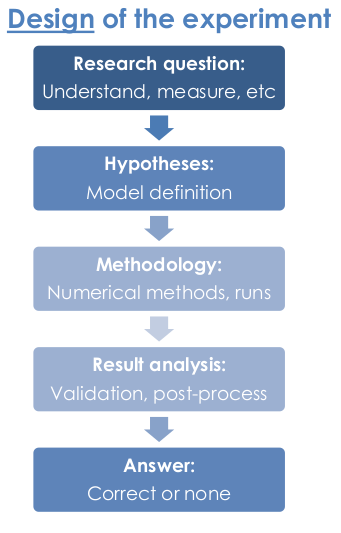
\includegraphics[width=0.3\textwidth]{Images/designExp}
    \caption{Illustration of the key aspects in the CFD simulation, interpreted as an experiment designed and performed to answer a fluid-dynamic question}
    \label{fig:cfdstep}
\end{figure}

Thanks to the \texttt{\textbackslash subfloat} command, a single figure, such as Figure~\ref{fig:quadtree2},
can contain multiple sub-figures with their own caption and label, e.g. Figure~\ref{fig:polimi_logo1} and Figure~\ref{fig:polimi_logo2}. 

\begin{figure}
    \centering
    \subfloat[One PoliMi logo.\label{fig:polimi_logo1}]{
        
\includegraphics[scale=0.5]{Images/logo_polimi_scritta}
    }
    \quad
    \subfloat[Another one PoliMi logo.\label{fig:polimi_logo2}]{
        
\includegraphics[scale=0.5]{Images/logo_polimi_scritta2}
    }
    \caption[]{Caption of the Figure.}
    \label{fig:quadtree2}
\end{figure}

\subsection{Tables example}
\label{subsec:tables}
Within the environments \texttt{table} and  \texttt{tabular} you can create very fancy tables as the one shown in Table~\ref{table:example}.
\begin{table}
    \caption{Caption of the Table.}
    \centering 
    \begin{tabular}{c c c }
    \toprule
    column1 & column2 & column3\\
    \midrule
    1 & 2 & 3 \\
    $\alpha$ & $\beta$ & $\gamma$ \\
    alpha & beta & gamma \\
    \bottomrule
    \end{tabular}
    \label{table:example}
\end{table}

\subsection{Lists}
How to insert itemized lists:
\begin{itemize}
    \item first item;
    \item second item.
\end{itemize}
How to write numbered lists:
\begin{enumerate}
    \item first item;
    \item second item.
\end{enumerate}

\vspace{0.3cm} % Insert vertical space

\subsection{Use of copyrighted material}
Each student is responsible for obtaining copyright permissions, if necessary, to include published material in the report.
This applies typically to third-party material published by someone else.

\subsection{Plagiarism}
You have to be sure to respect the rules on Copyright and avoid involuntary plagiarism.
It is allowed to take other persons' ideas only if the author and his original work are clearly mentioned.
As stated in the Code of Ethics and Conduct, Politecnico di Milano \textit{promotes the integrity of research,
condemns manipulation and the infringement of intellectual property}, and gives opportunity to all those
who carry out research activities to have an adequate training on ethical conduct and integrity while doing research.
To be sure to respect the copyright rules, read the guides on Copyright legislation and citation styles available
at:
\begin{verbatim}
https://www.biblio.polimi.it/en/tools/courses-and-tutorials
\end{verbatim}
You can also attend the courses which are periodically organized on "Bibliographic citations and bibliography management".

%-------------------------------------------------------------------------
%	END OF YOUR DOCUMENT
%-------------------------------------------------------------------------
\end{document}

